\thispagestyle{fancy}
\begin{center}
	\LARGE{\textbf{Resistores en paralelo}}
\end{center}
\section{Objetivos}
Al final de esta experiencia, uted. Podrá:
\begin{enumerate}
	\item Conectar resistores en distintos circuitos paralelo. 
	\item Usar el multimetro para medir la conductancia de varios circuitos en paralelo
\end{enumerate} 
\section{Conocimientos previos}
Dos resistores se hallan en paralelo cuando sus bornes estan conectados a un mismo nodo. Por lo tanto, la caída de tensión es la misma en cada uno de los resistores. 
\begin{figure}[h]
	\centering
	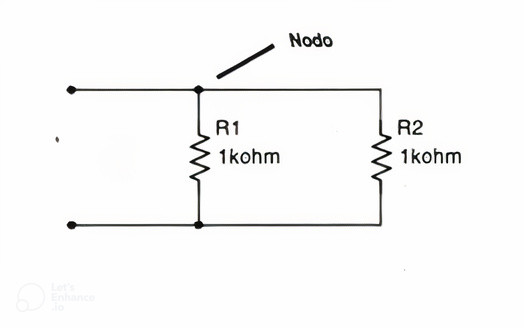
\includegraphics[scale=0.5]{imagenes/2}
	\caption{Circuito modelo}
\end{figure}
\\
Un grupo de resistores en paralelo siempre puede reemplazarse por un solo resistor equivalente $R_{eq}$.
Para dos resistores en paralelo, la resistencia equivalente se calcula como: 
\begin{equation*}
	R_{p}=\frac{R_{1} xR_{2}}{R_{1}+R_{2} }
\end{equation*}
Para calcular los equivalentes de mas de dos resistores en paralelo, deben convertirse a sus conductancias por medio de la relacion: 
\begin{equation*}
	conductancia=\frac{1}{Resistencia}    
\end{equation*}
\begin{equation*}
	 G= \frac{1}{R}
\end{equation*}
Entonces use la ecuación: 
\begin{equation*}
	G_{p}= G_{1} + G_{2} + G_{3} + . . . + G_{n}
\end{equation*}
Finalmente, la resistencia equivalente se calcula convirtiendo $G_{p}$a $R_{p}$.
\section{Autoevaluación de entrada}
\begin{enumerate}
	\item La resistencia equivalente de un conjunto de resistores conectados en paralelo es:
	\\
	La inversa de la resistencia equivalente es igual a la suma de las inversas de las resistencias $\frac{1}{R_{e}} =\frac{1}{R_{2}} + \frac{1}{R_{3}} + \frac{1}{R_{4}} +\frac{1}{R_{5}} + . . . + \frac{1}{R_{n}}$ 
	\item La caída de tencion en resistencias conectadas en paralelo es igual a:
	\\ 
	Suponiendo que la tensión de un circuito que tiene dos resistencias en paralelo es un voltaje V, entonces la tensión de la resistencia $R_{1}$ y la resistencia $R_{2}$ es son iguales.	
\end{enumerate}
\section{Equipo}
El siguiente equipo es necesario para realizar del experimento.
\begin{enumerate}
	\item Modulo de experimentos 
	\item DMM (multimetro digital)
\end{enumerate}
\section{Procedimiento}
\begin{enumerate}
	\item Localice los circuitos que contiene los resistores $R_{1}, R_{2}$ y $R_{3}$
	\item Use el DMM para medir los valores de  $R_{1}, R_{2}$ y $R_{3}$. Anote sus resultados.
	\begin{table}[h]
		\centering
		\begin{tabular}{|c|c|c|c|}
			\hline
			&$R_{1}$&$R_{2}$&$R_{3}$\\
			\hline
			Valor nominal&$10k\Omega$&$20k\Omega$&$30k\Omega$\\
			\hline
			Valor medido&$9.95k\Omega$&$20.09k\Omega$&$30.07k\Omega$\\
			\hline
		\end{tabular}
	\end{table}
	\item 	Estudie y efectué los cálculos de la figura 10.1 
	\begin{equation*}
		R_{e}= \frac{R_{1}*R_{2}}{R_{1}+R_{2}} = \frac{1*1}{1+1}= \frac{1}{2}\Omega
	\end{equation*}
	\item Conecte $R_{1}$ y $R_{2}$ en paralelo: 
	\begin{figure}[h]
		\centering
		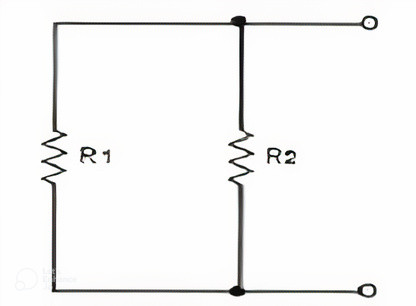
\includegraphics[scale=0.5]{imagenes/5.4}
		\caption{Circuito modelo}
	\end{figure}
	\item Mida y anote en la tabla la resistencia total de la combinación en paralelo.
	\\
	Resistencia paralelo de $R_{1}$ y $R_{2}=6.6667\Omega$
	\item Conecte $R_{1}$ y $R_{3}$ en paralelo. Mida y anote la resistencia en paralelo. Repita el procedimiento para $R_{2}$ y $R_{3}$.
	\\
	Resistencia en paralelo de$R_{1}$ y $R_{3}=7.5\Omega$ y resistencia en paralelo de $R_{2}$ y $R_{3}=12\Omega$
	\item Conecte en paralelo $R_{1}, R_{2}$ y $R_{3}$ Mida e registre la resistencia en paralelo:
	\\
	Resistencia en paralelo de $R_{1}, R_{2}$ y $R_{3}=5.4545\Omega$
	En esta parte del experimento, el circuito sufrirá modificaciones. 
	\item El valor de $R_{1}$ ha sido cambiado. Mida y anote la nueva resistencia equivalente de la conexión paralelo de  $R_{1}$ y $R_{2}$.
	\\ El valor en paralelo de $R_{1}$ y $R_{2}$ es igual a $2.7k\Omega$.
	\item Calcule el nuevo valor de $R_{1}$ usando la ecuación: 
	\begin{equation*}
		R_{1}=\frac{R_{p}*R_{2}}{R_{2}-R_{p}}=\frac{2.7*20}{20-2.7}=3.121387k\Omega
	\end{equation*}
	\\
	Conecte $R_{1}, R_{2}$ y $R_{3}$ en paralelo. Conéctelos a la fuente de alimentación PS-1. Fije la tensión de salida en 6V.
	\\
	Mida la corriente en cada resistor, así como la corriente total proveniente de la fuente de alimentación PS-1. Registre sus resultados.
	\begin{table}[h]
		\centering
		\begin{tabular}{|c|c|}
			\hline
			&Corriente (mA)\\
			\hline
			$R_{1}$& 1.92 mA\\
			\hline
			$R_{2}$& 0.30 mA\\
			\hline
			$R_{3}$& 0.2 mA\\
			\hline
			Total&2.42 mA\\
			\hline
		\end{tabular}
	\end{table}
\end{enumerate}
\section{Autoevaluación}
\begin{enumerate}
	\item Al cortocircuitar un resistor en un arreglo en paralelo causa:
	\\
	Causaría una disminución en la resistencia total del arreglo y un aumento en la corriente total que fluye a través del circuito.
	\item Al desconectar un resistor en un arreglo paralelo:
	\\
	Un aumento en la resistencia total del arreglo. 
\end{enumerate}
\section{Conclusión}
En este laboratorio se llego a calcular la resistencia equivalente de un circuito con resistores paralelos, como estos influyen en la corriente y caída de tensión del circuito.
\section{Anexos}

	\begin{figure}[h]
		\begin{minipage}{0.5\textwidth}
			\centering
			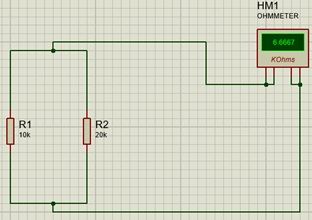
\includegraphics[width=0.8\linewidth]{imagenes/8}
			\caption{Medición 1}
		\end{minipage}%
		\begin{minipage}{0.5\textwidth}
			\centering
			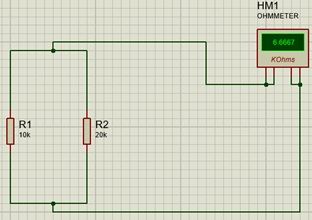
\includegraphics[width=0.8\linewidth]{imagenes/9}
			\caption{Medición 2}
		\end{minipage}
	\end{figure}
	
	\begin{figure}[h]
		\begin{minipage}{0.5\textwidth}
			\centering
			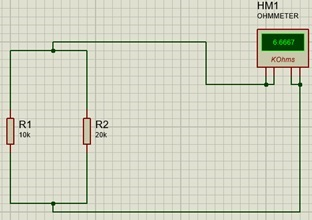
\includegraphics[width=0.8\linewidth]{imagenes/10}
			\caption{Medición 3}
		\end{minipage}%
		\begin{minipage}{0.5\textwidth}
			\centering
			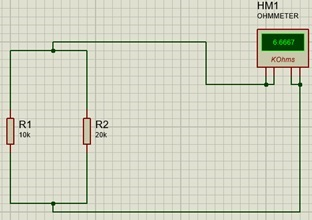
\includegraphics[width=0.8\linewidth]{imagenes/11}
			\caption{Medición 4}
		\end{minipage}
	\end{figure}
	
	\begin{figure}[h]
		\begin{minipage}{0.5\textwidth}
			\centering
			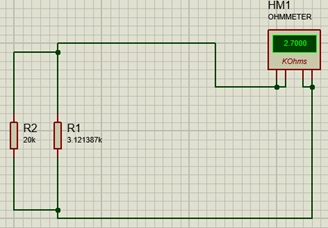
\includegraphics[width=0.8\linewidth]{imagenes/12}
			\caption{Medición 5}
		\end{minipage}%
		\begin{minipage}{0.5\textwidth}
			\centering
			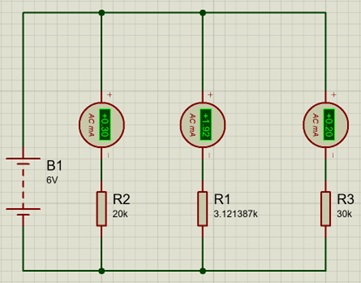
\includegraphics[width=0.8\linewidth]{imagenes/13}
			\caption{Medición 6}
		\end{minipage}
	\end{figure}

